\documentclass[nofonts,]{tufte-handout}

% ams
\usepackage{amssymb,amsmath}

\usepackage{ifxetex,ifluatex}
\usepackage{fixltx2e} % provides \textsubscript
\ifnum 0\ifxetex 1\fi\ifluatex 1\fi=0 % if pdftex
  \usepackage[T1]{fontenc}
  \usepackage[utf8]{inputenc}
\else % if luatex or xelatex
  \makeatletter
  \@ifpackageloaded{fontspec}{}{\usepackage{fontspec}}
  \makeatother
  \defaultfontfeatures{Ligatures=TeX,Scale=MatchLowercase}
  \makeatletter
  \@ifpackageloaded{soul}{
     \renewcommand\allcapsspacing[1]{{\addfontfeature{LetterSpace=15}#1}}
     \renewcommand\smallcapsspacing[1]{{\addfontfeature{LetterSpace=10}#1}}
   }{}
  \makeatother
\fi

% graphix
\usepackage{graphicx}
\setkeys{Gin}{width=\linewidth,totalheight=\textheight,keepaspectratio}

% booktabs
\usepackage{booktabs}

% url
\usepackage{url}

% hyperref
\usepackage{hyperref}

% units.
\usepackage{units}


\setcounter{secnumdepth}{-1}

% citations
\usepackage{natbib}
\bibliographystyle{plainnat}

%% tint override
\setcitestyle{round} 

% pandoc syntax highlighting

% longtable
\usepackage{longtable,booktabs}

% multiplecol
\usepackage{multicol}

% strikeout
\usepackage[normalem]{ulem}

% morefloats
\usepackage{morefloats}


% tightlist macro required by pandoc >= 1.14
\providecommand{\tightlist}{%
  \setlength{\itemsep}{0pt}\setlength{\parskip}{0pt}}

% title / author / date
\title{Selection Methods for Cross Pollinated Crops}
\author{Deependra Dhakal}
\date{2020-06-28}

%% -- tint overrides
%% fonts, using roboto (condensed) as default
\usepackage[sfdefault,condensed]{roboto}
%% also nice: \usepackage[default]{lato}

%% colored links, setting 'borrowed' from RJournal.sty with 'Thanks, Achim!'
\RequirePackage{color}
\definecolor{link}{rgb}{0.1,0.1,0.8} %% blue with some grey
\hypersetup{
  colorlinks,%
  citecolor=link,%
  filecolor=link,%
  linkcolor=link,%
  urlcolor=link
}

%% macros
\makeatletter

%% -- tint does not use italics or allcaps in title
\renewcommand{\maketitle}{%     
  \newpage
  \global\@topnum\z@% prevent floats from being placed at the top of the page
  \begingroup
    \setlength{\parindent}{0pt}%
    \setlength{\parskip}{4pt}%
    \let\@@title\@empty
    \let\@@author\@empty
    \let\@@date\@empty
    \ifthenelse{\boolean{@tufte@sfsidenotes}}{%
      %\gdef\@@title{\sffamily\LARGE\allcaps{\@title}\par}%
      %\gdef\@@author{\sffamily\Large\allcaps{\@author}\par}%
      %\gdef\@@date{\sffamily\Large\allcaps{\@date}\par}%
      \gdef\@@title{\begingroup\fontseries{b}\selectfont\LARGE{\@title}\par}%
      \gdef\@@author{\begingroup\fontseries{l}\selectfont\Large{\@author}\par}%
      \gdef\@@date{\begingroup\fontseries{l}\selectfont\Large{\@date}\par}%
    }{%
      %\gdef\@@title{\LARGE\itshape\@title\par}%
      %\gdef\@@author{\Large\itshape\@author\par}%
      %\gdef\@@date{\Large\itshape\@date\par}%
      \gdef\@@title{\begingroup\fontseries{b}\selectfont\LARGE\@title\par\endgroup}%
      \gdef\@@author{\begingroup\fontseries{l}\selectfont\Large\@author\par\endgroup}%
      \gdef\@@date{\begingroup\fontseries{l}\selectfont\Large\@date\par\endgroup}%
    }%
    \@@title
    \@@author
    \@@date
  \endgroup
  \thispagestyle{plain}% suppress the running head
  \tuftebreak% add some space before the text begins
  \@afterindentfalse\@afterheading% suppress indentation of the next paragraph
}

%% -- tint does not use italics or allcaps in section/subsection/paragraph
\titleformat{\section}%
  [hang]% shape
  %{\normalfont\Large\itshape}% format applied to label+text
  {\fontseries{b}\selectfont\Large}% format applied to label+text
  {\thesection}% label
  {1em}% horizontal separation between label and title body
  {}% before the title body
  []% after the title body

\titleformat{\subsection}%
  [hang]% shape
  %{\normalfont\large\itshape}% format applied to label+text
  {\fontseries{m}\selectfont\large}% format applied to label+text
  {\thesubsection}% label
  {1em}% horizontal separation between label and title body
  {}% before the title body
  []% after the title body

\titleformat{\paragraph}%
  [runin]% shape
  %{\normalfont\itshape}% format applied to label+text
  {\fontseries{l}\selectfont}% format applied to label+text
  {\theparagraph}% label
  {1em}% horizontal separation between label and title body
  {}% before the title body
  []% after the title body

%% -- tint does not use italics here either
% Formatting for main TOC (printed in front matter)
% {section} [left] {above} {before w/label} {before w/o label} {filler + page} [after]
\ifthenelse{\boolean{@tufte@toc}}{%
  \titlecontents{part}% FIXME
    [0em] % distance from left margin
    %{\vspace{1.5\baselineskip}\begin{fullwidth}\LARGE\rmfamily\itshape} % above (global formatting of entry)
    {\vspace{1.5\baselineskip}\begin{fullwidth}\fontseries{m}\selectfont\LARGE} % above (global formatting of entry)
    {\contentslabel{2em}} % before w/label (label = ``II'')
    {} % before w/o label
    {\rmfamily\upshape\qquad\thecontentspage} % filler + page (leaders and page num)
    [\end{fullwidth}] % after
  \titlecontents{chapter}%
    [0em] % distance from left margin
    %{\vspace{1.5\baselineskip}\begin{fullwidth}\LARGE\rmfamily\itshape} % above (global formatting of entry)
    {\vspace{1.5\baselineskip}\begin{fullwidth}\fontseries{m}\selectfont\LARGE} % above (global formatting of entry)
    {\hspace*{0em}\contentslabel{2em}} % before w/label (label = ``2'')
    {\hspace*{0em}} % before w/o label
    %{\rmfamily\upshape\qquad\thecontentspage} % filler + page (leaders and page num)
    {\upshape\qquad\thecontentspage} % filler + page (leaders and page num)
    [\end{fullwidth}] % after
  \titlecontents{section}% FIXME
    [0em] % distance from left margin
    %{\vspace{0\baselineskip}\begin{fullwidth}\Large\rmfamily\itshape} % above (global formatting of entry)
    {\vspace{0\baselineskip}\begin{fullwidth}\fontseries{m}\selectfont\Large} % above (global formatting of entry)
    {\hspace*{2em}\contentslabel{2em}} % before w/label (label = ``2.6'')
    {\hspace*{2em}} % before w/o label
    %{\rmfamily\upshape\qquad\thecontentspage} % filler + page (leaders and page num)
    {\upshape\qquad\thecontentspage} % filler + page (leaders and page num)
    [\end{fullwidth}] % after
  \titlecontents{subsection}% FIXME
    [0em] % distance from left margin
    %{\vspace{0\baselineskip}\begin{fullwidth}\large\rmfamily\itshape} % above (global formatting of entry)
    {\vspace{0\baselineskip}\begin{fullwidth}\fontseries{m}\selectfont\large} % above (global formatting of entry)
    {\hspace*{4em}\contentslabel{4em}} % before w/label (label = ``2.6.1'')
    {\hspace*{4em}} % before w/o label
    %{\rmfamily\upshape\qquad\thecontentspage} % filler + page (leaders and page num)
    {\upshape\qquad\thecontentspage} % filler + page (leaders and page num)
    [\end{fullwidth}] % after
  \titlecontents{paragraph}% FIXME
    [0em] % distance from left margin
    %{\vspace{0\baselineskip}\begin{fullwidth}\normalsize\rmfamily\itshape} % above (global formatting of entry)
    {\vspace{0\baselineskip}\begin{fullwidth}\fontseries{m}\selectfont\normalsize\rmfamily} % above (global formatting of entry)
    {\hspace*{6em}\contentslabel{2em}} % before w/label (label = ``2.6.0.0.1'')
    {\hspace*{6em}} % before w/o label
    %{\rmfamily\upshape\qquad\thecontentspage} % filler + page (leaders and page num)
    {\upshape\qquad\thecontentspage} % filler + page (leaders and page num)
    [\end{fullwidth}] % after
}{}

  
\makeatother


\usepackage{booktabs}
\usepackage{longtable}
\usepackage{array}
\usepackage{multirow}
\usepackage{wrapfig}
\usepackage{float}
\usepackage{colortbl}
\usepackage{pdflscape}
\usepackage{tabu}
\usepackage{threeparttable}
\usepackage{threeparttablex}
\usepackage[normalem]{ulem}
\usepackage{makecell}
\usepackage{xcolor}
\usepackage{tikz}
\usepackage{pgfplots}
\pgfplotsset{compat=1.16}
\usepackage{smartdiagram}
\usetikzlibrary{shapes.geometric,intersections}

\begin{document}

\maketitle




\clearpage

\hypertarget{introduction}{%
\section{Introduction}\label{introduction}}

\citep{posselt2010breeding} provides a detailed overview of breeding
methods commonly used in Cross Pollinated species. The text found basis
on the systematics of breeding explained by \citet{schnell1982synoptic}.

Breeding methods are specific, not so much to crops, but rather to modes
of reproduction and to types of varieties to be bred. According to
propagational type of the resulting varieties breeding methods can be
classified into four breeding categories: Line, population, hybrid and
clone.

\vspace{1cm}

\begin{figure}
\centering
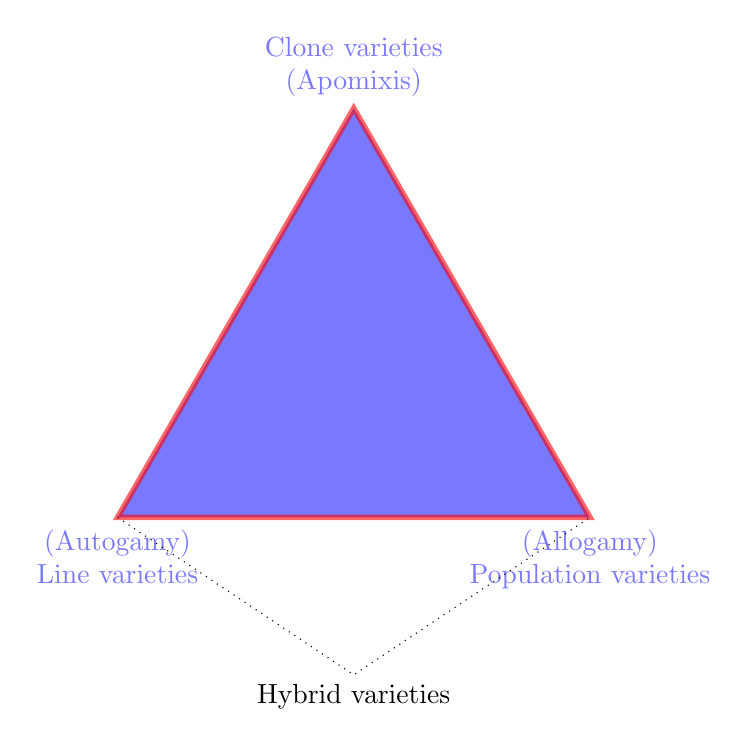
\begin{tikzpicture}
\coordinate (A) at (1,0);
\coordinate (B) at (4,{sqrt(27)});
\coordinate (C) at (7,0);
<!-- % \draw[step=0.5cm,color=gray] (0,-3) grid (8,6); -->
\draw[name path=UP, fill, color=blue!88, draw=red, line width=2pt,opacity=0.6]
(A) node[anchor=north,align=center]{(Autogamy)\\ Line varieties} -- (C) node[anchor=north,align=center]{(Allogamy)\\ Population varieties} -- (B) node[anchor=south,align=center]{Clone varieties\\ (Apomixis)} -- cycle;
\draw[name path=DOWN,dotted] (A)--(4,-2) node[anchor=north,align=center]{Hybrid varieties}--(C);
<!-- % using name path requires intersections tikzlibrary -->
\end{tikzpicture}
\caption{The reproduction triangle with the modes of reproduction (in bracketted letters) and the four breeding categories and resulting types of varieties. The system also imples that thare are not strict barriers between reproductive systems, but a gradual transition from one mode to the neighboring one. Clonal varieties can be selected for strictly apomictic plants. While autogamy and allogamy are not as strict in plant kingdom as even highly autogamous lines may cross fertilize nearby plants. Hybrid breeding, as shown involves both autogamy and allogamy and could be called a man-made breeding system.} \label{fig:triangle-of-breeding}
\end{figure}

Four types of varieties mentioned above can be grouped according to
their genetic and phenotypic variability (homogeneity or heterogeneity)
and their genetic constitution (homozygous or heterozygous). Maximum
heterozygosity can be achieved in single-cross hybrids.

\hypertarget{breeding-population-varieties}{%
\subsection{Breeding Population
Varieties}\label{breeding-population-varieties}}

According to \citet{schnell1982synoptic}, two types of population
varieties can be distinguished: OPVs and Synthetics.

\marginnote{\textbf{OPVs}: The result of population improvement through recurrent selection, and synthetic varieties.}

\marginnote{\textbf{Synthetics}: A commercial synthetic variety is an advanced generation of a population initiated by crosses among a restricted number of [GCA] selected parents and multiplied by a number of random out-crossing in isolation}

Both OPVs and synthetic varieties constitute panmictic populations,
since they are produced by random fertilization, at least in the
advanced generations of seed production.

To structure breeding methods, partitioning of breeding into three
phases will be helpful:

\begin{enumerate}
\def\labelenumi{\arabic{enumi}.}
\item
  Procuring intitial variation: This step creates a base population for
  imposing selection. If non-adapted materials shall be used,
  pre-breeding methods may be necessary beforehand.
\item
  Forming varietal parents: It comprises selection of the best
  individuals as the immediate parents of the first generation used to
  construct experimental varieties, or to create an improved breeding
  population. Since the likelihood of success after one step of
  selection is rather poor, population improvement through recurrent
  selection is typical in population breeding and is inevitable for
  future breeding progress.
\item
  Testing experimental varieties: Experimental varieties are constructed
  and tested. In this phase, procedures differ between schemes of OPV
  and synthetic breeding.
\end{enumerate}

\marginnote{Principe source materials are:
\newline 1. Wild types
\newline 2. Ecotypes (from own collections or genebanks)
\newline 3. Landraces
\newline 4. Improved breeding materials (populations, families, clones, inbreds)
\newline 5. Released varieties (OPVs, synthetics)}

\newthought{Choice of germplasm is a critical decision that requires considerable thought. Hasty decisions either to eliminate or to decrease number of growing seasons required may in the long run increase the number of growing seasons required to develop usable materials. In many instances the selected germplasm will be the basis of the breeding program for the lifetime of the breeder. Choice of germplasm will determine maximum potential improvement that can be attained via breeding; the breeding system used will determine how much of that maximum potential can be realized.}

\hfill Haullauer and Miranda (1981)

Breeder faces several problems of choice regarding creating of base
population:

\begin{itemize}
\tightlist
\item
  Whether to establish one or several base populations,
\item
  Use of base population in short-term or long-term selection programmes
\item
  Whether to allow open population or maintain closed population
\end{itemize}

\marginnote{Mostly for research studies, closed populations are used.$$\frac{d}{dx}\left( \int_{a}^{x} f(u)\,du\right)=f(x)$$.}

\clearpage

\renewcommand\refname{References}
\bibliography{cross-pollinated-crops.bib}



\end{document}
